\ifx\mainfile\undefined
%  ========================================================================
%  Copyright (c) 2006-2011 The University of Washington
%
%  Licensed under the Apache License, Version 2.0 (the "License");
%  you may not use this file except in compliance with the License.
%  You may obtain a copy of the License at
%
%      http://www.apache.org/licenses/LICENSE-2.0
%
%  Unless required by applicable law or agreed to in writing, software
%  distributed under the License is distributed on an "AS IS" BASIS,
%  WITHOUT WARRANTIES OR CONDITIONS OF ANY KIND, either express or implied.
%  See the License for the specific language governing permissions and
%  limitations under the License.
%  ========================================================================
%
 
\documentclass [11pt, twoside] {uwthesis}

\usepackage{color}
\usepackage{url}
\usepackage{amsmath}
\usepackage{amsfonts}
\usepackage[bookmarks,
	hidelinks,
	plainpages=false,
	pdfpagelabels,
	pagebackref=true,
            ]{hyperref}
\renewcommand*{\backref}[1]{}% for backref < 1.33 necessary
\renewcommand*{\backrefalt}[4]{%
  \ifcase #1 %
    (No citations.)%
  \or
    (Cited on page #2.)%
  \else
    (Cited on pages #2.)%
  \fi
}

\newcommand{\biburl}[1]{{\tt<}\url{#1}{\tt>}}

\hypersetup{%
pdfauthor = {Daniel Chaim Halperin},
pdftitle = {Simplifying the Configuration of 802.11 Wireless Networks with Effective SNR},
pdfsubject = {Ph.D. Dissertation},
pdfkeywords = {},
pdfcreator = {University of Washington, Computer Science and Engineering},
pdfproducer = {},
bookmarksopen = {true},
pdfpagelayout = {TwoColumnRight},
}

\usepackage{footnotebackref}
%%%%%%%%%%%%%%%%%%%%%%%%%%%%%%%%%%%%%%%%%%%%%%%%%%%%%%
%%%        Formatting sections                     %%%
%%%%%%%%%%%%%%%%%%%%%%%%%%%%%%%%%%%%%%%%%%%%%%%%%%%%%%
\newcommand{\algref}[1]{Algorithm~\ref{#1}}
\newcommand{\chapref}[1]{Chapter~\ref{#1}}
\renewcommand{\eqref}[1]{Equation~\ref{#1}}
\newcommand{\figref}[1]{Figure~\ref{#1}}
\newcommand{\secref}[1]{\S\ref{#1}}
\newcommand{\tabref}[1]{Table~\ref{#1}}
\newcommand{\heading}[1]{\vspace{4pt}\noindent\textbf{#1}}
\newcommand{\topheading}[1]{\noindent\textbf{#1}}
\newcommand{\noheading}[0]{\vspace{4pt}\noindent}

%%%%%%%%%%%%%%%%%%%%%%%%%%%%%%%%%%%%%%%%%%%%%%%%%%%%%%
%%%        XXX and other warnings                  %%%
%%%%%%%%%%%%%%%%%%%%%%%%%%%%%%%%%%%%%%%%%%%%%%%%%%%%%%
\newcommand{\xxx}[1]{\textit{\color{red}XXX #1}}

%%%%%%%%%%%%%%%%%%%%%%%%%%%%%%%%%%%%%%%%%%%%%%%%%%%%%%
%%%        Units                                   %%%
%%%%%%%%%%%%%%%%%%%%%%%%%%%%%%%%%%%%%%%%%%%%%%%%%%%%%%
\usepackage{xspace}
\newcommand{\unitsep}{\texorpdfstring{\,}{ }}
\def\unit#1{% from: http://www.tex.ac.uk/cgi-bin/texfaq2html?label=csname "Defining a macro from an argument"
  \expandafter\def\csname #1\endcsname{\unitsep\text{#1}\xspace}%
}
\def\varunit#1#2{% from: http://www.tex.ac.uk/cgi-bin/texfaq2html?label=csname "Defining a macro from an argument"
  \expandafter\def\csname #1\endcsname{\unitsep\text{#2}\xspace}%
}
\unit{GHz}
\unit{MHz}
\unit{kHz}
\unit{Gbps}
\unit{Mbps}
\unit{KB}
\unit{dB}
\unit{dBi}
\unit{dBm}
\unit{W}
\unit{mW}
\varunit{uW}{$\mu$W}
\unit{ms}
\varunit{us}{$\mu$s}
\unit{h}
\unit{m}
\unit{s}
\unit{km}
\unit{cm}
\unit{mm}
\varunit{mmsq}{mm$^\text{2}$}
\varunit{insq}{in$^\text{2}$}
\newcommand{\degree}{\ensuremath{^\circ}\xspace}
\newcommand{\degrees}{\degree}
%%%%%%%%%%%%%%%%%%%%%%%%%%%%%%%%%%%%%%%%%%%%%%%%%%%%%%%%%%%%%%%%%%%%%%%%%%%%%%%%%%%%%%
% Euler for math | Palatino for rm | Helvetica for ss | Courier for tt
%
% From: http://www.tug.org/mactex/fonts/LaTeX_Preamble-Font_Choices.html
%%%%%%%%%%%%%%%%%%%%%%%%%%%%%%%%%%%%%%%%%%%%%%%%%%%%%%%%%%%%%%%%%%%%%%%%%%%%%%%%%%%%%%
\renewcommand{\rmdefault}{ppl} % rm
\usepackage[scaled]{helvet} % ss
\usepackage{courier} % tt
\usepackage{eulervm} % a better implementation of the euler package (not in gwTeX)
\normalfont
\usepackage[T1]{fontenc}
%%%%%%%%%%%%%%%%%%%%%%%%%%%%%%%%%%%%%%%%%%%%%%%%%%%%%%%%%%%%%%%%%%%%%%%%%%%%%%%%%%%%%%

%%%%%%%%%%%%%%%%%%%%%%%%%%%%%%%%%%%%%%%%%%%%%%%%%%%%%%
%%%        Figures                                 %%%
%%%%%%%%%%%%%%%%%%%%%%%%%%%%%%%%%%%%%%%%%%%%%%%%%%%%%%
\usepackage{graphicx}
% Caption package both lets you set the spacing between figure and caption
% and also makes the \figref{} point to the right place.
\usepackage[font=bf,aboveskip=6pt,belowskip=-4mm]{caption}
% Allow subfigures, make them bold
\usepackage[bf,BF,small]{subfigure}
% List of figures
\setcounter{lofdepth}{2}  % Print the chapter and sections to the lot

%%%%%%%%%%%%%%%%%%%%%%%%%%%%%%%%%%%%%%%%%%%%%%%%%%%%%%
%%%        Lists with reduced spacing              %%%
%%%%%%%%%%%%%%%%%%%%%%%%%%%%%%%%%%%%%%%%%%%%%%%%%%%%%%
\usepackage{enumitem}

%%%%%%%%%%%%%%%%%%%%%%%%%%%%%%%%%%%%%%%%%%%%%%%%%%%%%%
%%%        Fancy tables                            %%%
%%%%%%%%%%%%%%%%%%%%%%%%%%%%%%%%%%%%%%%%%%%%%%%%%%%%%%
\usepackage{tabulary}
\usepackage{booktabs}

%%%%%%%%%%%%%%%%%%%%%%%%%%%%%%%%%%%%%%%%%%%%%%%%%%%%%%
%%%        Formatting techniques/tools/etc.        %%%
%%%%%%%%%%%%%%%%%%%%%%%%%%%%%%%%%%%%%%%%%%%%%%%%%%%%%%
\newcommand{\term}[1]{\texttt{#1}}

\begin{document}
 
\textpages
\setcounter{chapter}{3} % Set to n-1!
\fi
%%%%%%%%%%%%%%%%%%%%%%%%%%%%%%%%%%

\cleardoublepage
\chapter{Model}
\label{chap:model}

\heading{802.11 Packet Reception.}
The model must account for the action of the 802.11 receiver on the received signal. This is a complex process described in many pages of the 802.11n specification~\cite{80211n}. Our challenge is to capture it well enough with a fairly simple model. We begin by describing the main steps involved (\figref{fig:ofdm_decoding}).

First, MIMO processing separates the signals of multiple spatial streams that have been mixed by the channel. As wireless channels are frequency-selective, this operation happens separately for each subcarrier. The demodulator converts each subcarrier's symbols into the bits of each stream from constellations of several different modulations (BPSK, QPSK, 16-QAM, 64-QAM). This happens in much the same way as demodulating a narrowband channel. The bits are then deinterleaved to undo an encoding that spreads errors that are bursty in frequency across the data stream. A parallel to serial converter combines the bits into a single stream. Forward error correction at any of several rates (1/2, 2/3, 3/4, and 5/6) is then decoded. Finally, the descrambler exclusive-ORs the bitstream with a pseudorandom bitmask added at the transmitter to avoid data-dependent deterministic errors.

\begin{figure*}[ht]
\centering
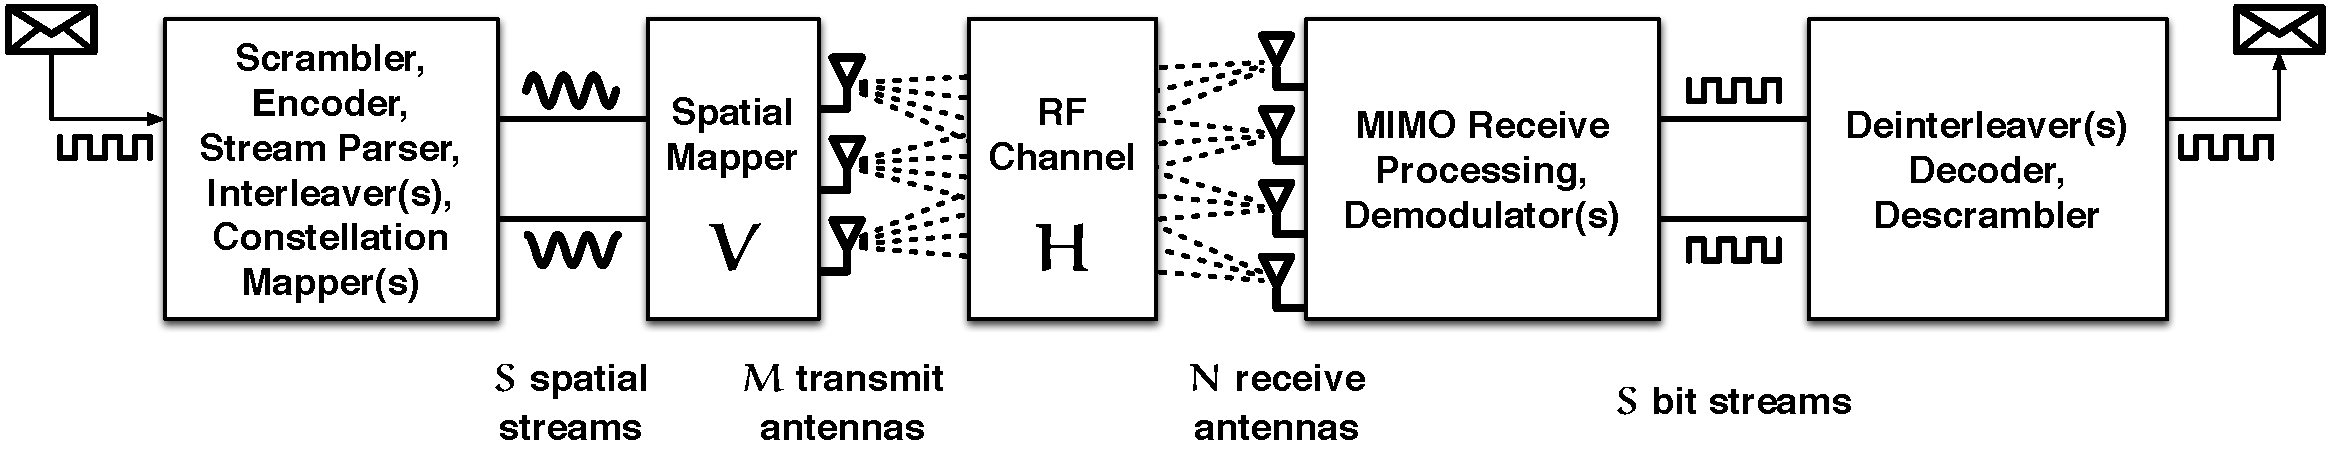
\includegraphics[width=\textwidth]{figures/11n_link_simplified_bigger_fonts.pdf}
\caption[An 802.11n link]{Caption goes here}
\end{figure*}

%\begin{figure*}[ht]
%\centering
%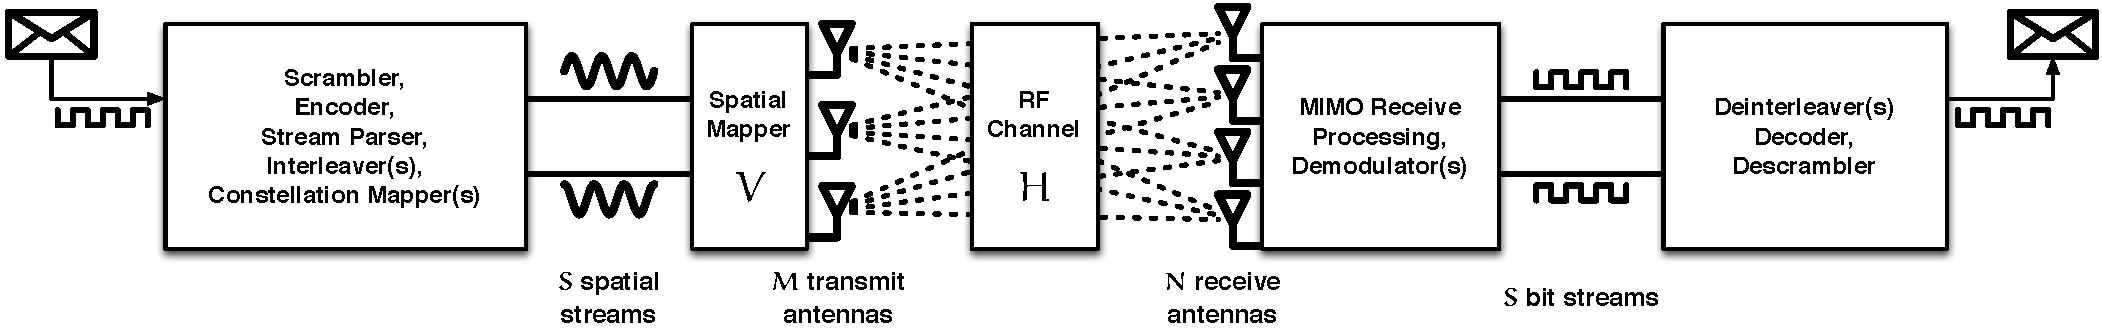
\includegraphics[angle=90,height=\textheight]{figures/11n_link_simplified.pdf}
%\caption[An 802.11n link]{Caption goes here}
%\end{figure*}

\begin{figure*}[ht!]
\centering
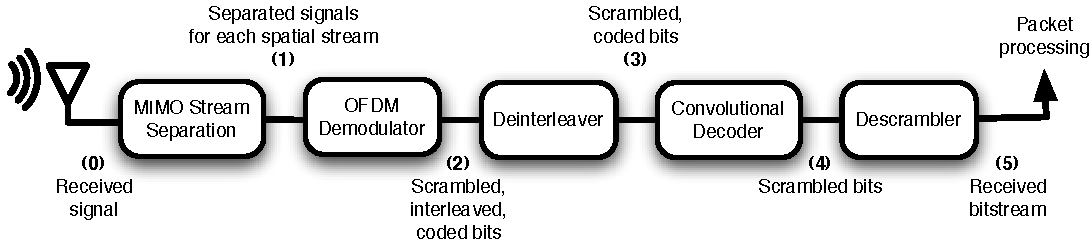
\includegraphics[width=6in]{figures/esnr/mimo_ofdm_decoding_process.pdf}
\caption[The 802.11n MIMO-OFDM decoding process]{\label{fig:ofdm_decoding} The 802.11n MIMO-OFDM decoding process. MIMO receiver separates the RF signal~(0) for each spatial stream~(1). Demodulation converts the separated signals into bits~(2). Bits from the multiple streams are deinterleaved and combined~(3) followed by convolutional decoding~(4) to correct errors. Finally, scrambling that randomizes bit patterns is removed and the packet is processed~(5).}
\end{figure*}

\begin{table}
\centering
%\footnotesize
\begin{tabular}{ccc}
\toprule
Modulation & Bits/Symbol ($k$) & BER$_k$($\rho$) \\
\midrule BPSK & 1 & $Q\left(\sqrt{2\rho}\right)$ \\
QPSK & 2 & $Q\left(\sqrt{\rho}\right)$\\
16-QAM & 4 & $\frac{3}{4}Q\left(\sqrt{\rho/5}\right)$\\
64-QAM & 6 & $\frac{7}{12}Q\left(\sqrt{\rho/21}\right)$\\
\bottomrule
\end{tabular}
\caption[Bit error rate as a function of the symbol SNR for OFDM modulations]{\label{tab:ber_snr}Bit error rate as a function of the symbol SNR $\rho$ for narrowband signals and OFDM modulations. $Q$ is the standard normal CDF\@.}
\end{table}

\heading{Modeling Delivery.}
We build our model up from narrowband demodulation. 
Standard formulas summarized in \tabref{tab:ber_snr} relate SNR (denoted $\rho$) to bit-error rate (BER) for the modulations used in 802.11~\cite{Goldsmith}. CSI gives us the SNR values ($\rho_s$) to use for each subcarrier. For a SISO system, $\rho_s$ is given by the single entry in $H_s$.

In OFDM, decoding is applied across the demodulated bits of subcarriers. If we assume frequency-flat fading for the moment, then all the subcarriers have the same SNR\@. The link will behave the same as in our wired experiments in which RSSI reflect real performance and it will be easy to make predictions for a given SNR and modulation combination. We can use \figref{fig:snr_prr_attenuator} to measure the fixed transition points between rates and thus make our choice.

Frequency-selective fading complicates this picture as some weak subcarriers will be much more likely to have errors than others that are stronger. To model a link in this case, we turn to the notion of an \textbf{\em Effective SNR}\@. This is defined as the SNR that would give the \emph{same error performance on a narrowband channel}~\cite{Nanda_EffectiveSNR}. For example, the links in \figref{fig:example_fsf_shape} will have Effective SNR values that are nearly equal because they perform similarly, even though their RSSIs are spread over 15\dB.

The Effective SNR is \emph{not} simply the average subcarrier SNR; indeed, assuming a uniform noise floor, that average is indeed equivalent to the packet SNR derived from the RSSI\@. Instead, the Effective SNR is biased towards the weaker subcarrier SNRs because it is these subcarriers that produce most of the errors. If we ignore coding for the moment, then we can compute the Effective SNR by averaging the subcarrier BERs and then finding the corresponding SNR\@. That is:
\begin{equation}
\label{eq:effective_ber}
	\text{BER}_{\text{eff},k} = \frac{1}{52} \sum \text{BER}_k(\rho_s)
\end{equation}
\begin{equation}
\label{eq:effective_snr}
	\rho_{\text{eff},k} = \text{BER}_k^{-1}(\text{BER}_{\text{eff},k})
\end{equation}
We use $\text{BER}_k^{-1}$ to denote the inverse mapping, from BER to SNR\@. We have also called the average BER across subcarriers the effective BER, $\text{BER}_{\text{eff}}$. SoftRate estimates BER using internal receiver state~\cite{Vutukuru_SoftRate}. We compute it from channel measurements instead.

Note that the BER mapping and hence Effective SNR are functions of the modulation ($k$). That is, unlike the RSSI, a particular wireless channel will have four different Effective SNR values, one describing performance for each of the modulations. In practice, the interesting regions for the four Effective SNRs do not overlap because at a particular Effective SNR value only one modulation will be near the transition from useless (BER $\approx$0.5) to lossless (BER $\approx$0). When graphs in this paper are presented with an Effective SNR axis, we use all four values, each in the appropriate SNR range.

For 802.11n, we also model MIMO processing at the receiver. To do this we need to estimate the subcarrier SNRs for each spatial stream from the channel state matrix $H_s$. Although the standard does not specify receiver processing, 
we assume that a Minimum Mean Square Error (MMSE) receiver is used. It is computationally simple, optimal and equivalent to Maximal-Ratio Combining (MRC) for a single stream, and near optimal for multiple streams. 
All of these make it a likely choice in practice.
%This assumption allows us to use standard formulas to map channel matrices for each subcarrier (from CSI) to per-stream subcarrier SNRs.
%The $N$ per-stream MMSE output SNRs for subcarrier $s$ are 
The SNR of the $i^{\text{th}}$ stream after MMSE processing for subcarrier $s$ is 
given by
\begin{equation}
\centering
\label{eq:mmse_snr}
\rho_{s,i} = \frac{1}{Y_{ii}}-1, \text{ where }
Y = \left(H_s^H H_s+I\right)^{-1}
\end{equation}
for $i \in [1,N]$ and $N$x$N$ identity matrix $I$~\cite{Tse}. For MIMO, the model computes the effective BER averaged across both subcarriers and streams.

Coding interacts with the notion of Effective SNR in a way that is difficult to analyze. One challenge is that the ability to correct bit errors depends on the position of the errors in the data stream. To sidestep this problem, we rely on the interleaving that randomizes the coded bits across subcarriers and spatial streams. Assuming perfect interleaving and robust coding, bit errors in the stream should look no different from bit errors for flat channels (but at a lower SNR). Thus our estimate of the effective BER in \eqref{eq:effective_ber} will accurately reflect the uncoded error performance of the link. Our algorithm now proceeds as in the case of a flat-fading channel described above: we take the computed Effective SNR value and use the measurements from a flat-fading link (\figref{fig:snr_prr_attenuator}) to determine transmission success or failure. As in CHARM~\cite{Judd_CHARM}, we support different packet lengths with different SNR thresholds.

Note that this procedure differs from the typical approach of simulation-based analyses~\cite{Kant_fla, Liu_EESM, Nortel_3g}, that instead map the \emph{uncoded} BER estimate such as we compute to a \emph{coded} BER estimate by means of a simple log-linear approximation. They then use the coded BER estimate, and the length of the target transmission, to directly compute the packet delivery rate of the link. We believe our method of thresholding the Effective SNR is better because it directly accommodates variation in the receiver implementation. Different devices may have different \emph{noise figures}, a measure of how much signal strength is lost in the internal RF circuitry of the NIC\@. They may implement soft Viterbi decoders with more or fewer soft bits for their internal state, or indeed might do hard decoding instead. A receiver could use the optimal Maximum Likelihood MIMO decoder that has exponential complexity for small constellations like BPSK, but revert to the imperfect but more efficient MMSE at higher modulations. All of these can be easily expressed, albeit maybe approximately, as (perhaps modulation-dependent) shifts in the Effective SNR thresholds. In contrast, changing these parameters in the simulation approach involves changing the internals of the calculation.

\heading{Protocol Details.} Effective SNR calculations can be performed by either receiver or transmitter, and each has advantages. For it to make decisions, the transmitter must know the receiver's thresholds for the different rates; these are fixed for a particular model of NIC and can be shared once, e.g., during association. The transmitter also needs up-to-date CSI: either from feedback or estimated from the reverse path. Alternately, the receiver can request rates and select antennas directly using the new Link Adaptation Control field of any 802.11n QoS packet~\cite[\S7.1.3.5a]{80211n}. This obviates sending CSI, but the calculation instead requires that the transmitter share its spatial mappings, i.e.\ how it maps spatial streams to transmit antennas. These are likely to change less frequently than the channel, if at all. Finally, when operating in either mode with fewer transmit streams than antennas, the transmitter must occasionally send a short probe packet with all antennas to measure the full CSI\@.

\heading{Summary and Example.} Combining the above steps, our model consists of the following: 1) CSI is obtained and a test configuration is chosen; 2) the MMSE expression is used to compute per-stream, subcarrier SNRs from the CSI for the test number of streams; 3) the Effective SNR is computed from the per-stream, subcarrier SNRs for the test modulation; and 4) the Effective SNR is compared against the pre-determined threshold for the test modulation and coding to predict whether the link will deliver packets.

\begin{figure}[t]
  \centering
  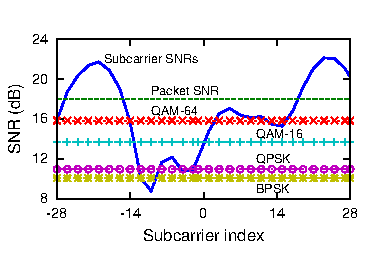
\includegraphics[width=0.9\columnwidth,viewport=0 9 180 111,clip]{figures/esnr/embed_fsf-shape-eff-snr-s3d5-txpower-20.pdf}
  % viewport=0 7 173 113
  \vspace{-4pt}
  \caption[Sample faded link showing the packet SNR and Effective SNRs for different modulations.]{Sample faded link showing the packet SNR and Effective SNRs for different modulations. BPSK has the lowest Effective SNR, but it needs less energy to decode.}
  \label{fig:eff_example}
  \vspace{-3pt}
\end{figure}


As an example, \figref{fig:eff_example} shows the CSI for a SISO link (steps 1--2) as a fading profile across subcarriers, with the computed Effective SNRs for all modulations (step 3). These Effective SNRs are compared with pre-determined thresholds (\figref{fig:snr_prr_attenuator}) to correctly predict that the best working rate will be 39\Mbps. 
Note that these Effective SNRs are well below the RSSI-based packet SNR that is biased towards the stronger subcarriers (note the logarithmic $y$-axis scale). This link does a poor job of harnessing the received power because it is badly faded, so its SNR is a poor predictor of rate.

\begin{table}
\begin{tabular}{ccccccc}
\toprule
\multirow{2}{*}{Algorithm} & \multirow{2}{*}{802.11a/b/g} & \multirow{2}{*}{MIMO} & Antenna & \multirow{2}{*}{TX Power} & Channel & \multirow{2}{*}{Real NICs} \\
& & & Selection & & Width \\
\midrule
SoftRate~\cite{Vutukuru_SoftRate} & \checkmark \\
AccuRate~\cite{Sen_AccuRate} & \checkmark & & & \checkmark & \checkmark \\
EEC~\cite{Chen_EEC} & \checkmark & & & & & \checkmark \\
Effective SNR & \checkmark & \checkmark & \checkmark & \checkmark & \checkmark & \checkmark\\
\bottomrule
\end{tabular}
\caption[Comparison of link error rate prediction algorithms]{\label{tab:algorithm_comparison}A comparison of Effective SNR to other recent algorithms that purport to predict the performance of a wireless link. Effective SNR can predict packet delivery in the largest space because it looks at the raw channel response, whereas the other techniques mostly apply only to single-stream links with fixed antennas and transmit power.}
\end{table}

%%%%%%%%%%%%%%%%%%%%%%%%%%%%%%%%%%
\ifx\mainfile\undefined
%
% ==========   Bibliography   ==========
%
%\nocite{*}   % include everything in the uwthesis.bib file
\bibliographystyle{plain}
\bibliography{dhalperi_thesis}

\end{document}
\fi
